\chapter{Related Work}
\label{ch:background}

%%%%%%%%%%%%%%%%%%%%%%%%%%%%%%%%%%%%%%%%%%%%%%%%%%%%%%%%%%%%%%%%%%%%%%%%%%%%%%%%%%%
%%%%%%%%%%%%%%%%%%%%%%%%%%%%%%%%%%%%%%%%%%%%%%%%%%%%%%%%%%%%%%%%%%%%%%%%%%%%%%%%%%%
%%%%%%%%%%%%%%%%%%%%%%%%%%%%%%%%%%%%%%%%%%%%%%%%%%%%%%%%%%%%%%%%%%%%%%%%%%%%%%%%%%%
%%%%%%%%%%%%%%%%%%%%%%%%%%%%%%%%%%%%%%%%%%%%%%%%%%%%%%%%%%%%%%%%%%%%%%%%%%%%%%%%%%%
%%%%%%%%%%%%%%%%%%%%%%%%%%%%%%%%%%%%%%%%%%%%%%%%%%%%%%%%%%%%%%%%%%%%%%%%%%%%%%%%%%%
\section{Part 1: Design-Time Network Analysis and Performance Prediction}
\label{sec:related_part1}

Networking systems have been developed for over half a century and the
analysis of processing networks and communications networks began even
earlier.  As computing power has increased, the field of network
performance analysis at design-time has evolved into two main
paradigms: (1) network performance testing of the applications and
system to be deployed to determine performance and pitfalls, and (2)
analytical models and techniques to provide application network
performance guarantees based on those models.  The first paradigm
generally involves either arbitrarily precise network simulation, or
network emulation, or sub-scale experiments on the actual system.  The
second paradigm focuses on formal models and methods for composing and
analyzing those models to derive performance predictions.

\subsection{Performance Analysis Through Network Simulation/Emulation}
\label{subsec:related_part1_simulation_emulation}

Since computing networks are so prevalent, many tools exist to analyze
system network behavior, either through simulation or mathematical
analysis, which both attempt to determine one or more system
properties based on one or more models of the system.  One method of
system simulation is discrete event
simulation\cite{devs_Schriber2013}, in which all relevant events in
the system are captured in the model and stepped through sequentially
with the state of the model changing only at the simulated time steps.
The resources of the system (e.g. buffer space) are simulated together
with the entities in the system (e.g. the bits of the network traffic)
through operations on the entities as they traverse the model and its
resources.  OMNET++\cite{omnet++} is a discrete event network
simulator which simulates the network traffic as it passes through the
network layers.  The INETMANET\cite{vagas2010inetmanet} framework,
built on top of OMNET++, supports the simulation of network traffic
over dynamic wireless links for gathering performance data about
applications on the network.

% ADD NS2/NS3 HERE
NS-2\cite{ns2_real_time2004} is a widely-used \textit{single-threaded}
discrete event simulator which allows both the simulation and
emulation of both wired and wireless networks.  Because of performance
and scalability issues, however, the simulator is not well suited for
scaling to large network simulation/emulation.  Furthermore, NS-2 has
simulation accuracy issues (e.g. altering event ordering or timing)
which plague any simulator used for emulation (i.e. connecting a
simulator to a system to emulate the subsystem it is
simulating). \cite{simulator_comparison_2003} gives a good study of
the accuracy of NS-2 simulation with a testbed and finds that for
constant bit-rate (CBR) traffic the simulation is accurate with
respect to the behavior of the real system testbed, but for other
types of traffic (e.g. FTP traffic), the simulation did not accurately
model the dynamic behavior of FTP traffic.

Despite the wide-spread use of these simulation toolsuites, it is
clear that they are not a viable candidate for providing both accurate
and precise design-time guarantees about network performance and
resource utilization.

% ADD EMULATION HERE
Instead of simulating the network/stack, another option is to directly
emulate the network by shaping the traffic between the actual nodes of
the system to directly apply the appropriate delay and enforce the
proper bandwidth on each link of the network.  Often this is done
through the use of flow control tools either on routing node(s) or on
capable network infrastructure devices, e.g. a smart switch.
Dummynet\cite{dummynet1997}\cite{dummynetRevisited2010} is a tool for
network emulation when used on routing nodes in a system, utilizing
the underlying network traffic shaping and policing tools available in
Linux.  Dummynet allows the configuration of routing tables, packet
drop rates, link bandwidths, and link delays to conform the traffic
passing through it to the supplied network configuration.
OpenFlow\cite{openflow2009openflow} is an alternative for network
emulation which instead uses a compatible smart switch to shape the
network traffic and enforce the proper network topology and
characteristics for all traffic in the network at a lower network
layer without requiring the use of a separate traffic shaping node.

For the types of systems we have described in Chapter~\ref{ch:intro},
typically these types of simulation and testbed emulation are used to
analyze the performance of the applications and the system.
Unfortunately simulation and emulation based performance analysis
techniques are unable to provide the guarantees required by
application developers and system integrators.

\subsection{Analytical Approaches to Network Analysis}
\label{subsec:related_part1_analytics}

\subsubsection{Queuing Theory}
% QUEUING THEORY HERE
Queuing Theory\cite{QT_Kendall1953}\cite{QT_Giambene2005} is a
probabilistic approach to the analysis of processing or communications
networks, and has been applied to many types of systems including
telecommunications, processing, and distribution systems.  A queuing
system can be described using notation of the form $A/B/S/\Delta/E$,
introduced by \cite{QT_Kendall1953}, with the semantics:
\begin{itemize}
	\item $A$: Type of arrival process, e.g. $M$ for Poisson Arrival Process
	\item $B$: Request service time statistics, e.g. $D$ for Deterministic service time
	\item $S$: Number of servers
	\item $\Delta$: Queue length
	\item $E$: Number of producers
\end{itemize}

Queuing Theory allows the analysis of the mean number of requests
($N$) in the queue and the mean buffering delay ($T$) experienced by
objects traversing the queue.  Little's Theorem provides the relation
between the two : $N=\lambda T$\cite{littleTheorem}, where $\lambda$
is the mean arrival rate into the queue.  However, this theorem
assumes (1) that the service policy is independent of service time and
(2) the service policy is work conserving.  Assumption (1) may be
violated for policy-based routing and servicing which tries to provide
guaranteed QoS to applications, and assumption (2) is violated by
wireless networks, in which nodes with very limited connectivity or
dropouts in connectivity are not able to service the data in the
buffers despite the existence of the data in the buffers and
applications continuing to produce data.

% MENTION HERE WHY QT ISN'T GREAT AND SET UP NC/RTC
For the types of systems we have described in Chapter~\ref{ch:intro},
probabilistic analysis techniques like Queuing Theory make providing
the requisite performance and resource guarantees difficult or
impossible because of the stochastic nature of the models of network
traffic\cite{NC_Cruz1991}.  Because of the need for these strict
guarantees, other deterministic formal models for the analysis of
communications and processing systems have been developed.

\subsubsection{Network Calculus and Min-Plus Calculus}
% SHORT INTRO TO NC HERE
Network Calculus\cite{NC_Cruz1991}\cite{NC_Cruz1991a}\cite{NCBook} is
a theory for deterministic queuing systems which provides the ability
to determine worst-case buffer requirements and application buffering
delay at design-time by applying the techniques of (min,+) calculus to
queuing theory.  We will describe the foundation of (min,+) calculus
before covering the techniques of Network Calculus. \cite{NCBook},
Chapter 3, gives an excellent overview of both min-plus and max-plus
calculus, on which Network Calculus is based.  An abbreviated
explanation of the concepts of these two related dioids (additive
inverses need not exist) follows.

Min-plus calculus, $(\mathbb{R}\cup\{+\infty\},\wedge,+)$, deals with \textit{wide-sense increasing functions} : 
\begin{equation}
\mathpzc{F}=\{f : \mathbb{R}^+ \rightarrow \mathbb{R}^+, \forall s \leq t : f(s) \leq f(t), f(0) = 0\}
\end{equation}
which represent functions whose slopes are always $\geq 0$.
Intuitively this makes sense for modeling network traffic, as data can
only ever by sent or not sent by the network, therefore the cumulative
amount of data sent by the network as a function of time can only ever
increase or stagnate.  A wide-sense increasing function can further be
classified as a sub-additive function if
\begin{equation}
\forall s,t : f(s+t) \leq f(s) + f(t)
\end{equation}
Note that if a function is concave with $f(0)=0$, it is sub-additive,
e.g. $y=\sqrt{x}$.  Sub-additivity of functions is required to be able
to define meaningful constraints for network calculus, though
realistically modeled systems (in Network Calculus) will always have
sub-additive functions to describe their network characteristics
(e.g. data serviced or data produced).  This sub-additivity comes from
the semantics of the modeling; since the models describe maximum data
production or minimum service as functions of \emph{time-windows},
maximum data production over a longer time window must inherently
encompass the maximum data production of shorter time-windows.  Some
examples of wide-sense increasing functions which are of use in
Network Calculus are shown in Figure~\ref{fig:wsi}.

\begin{figure}[htb]
	\centering
	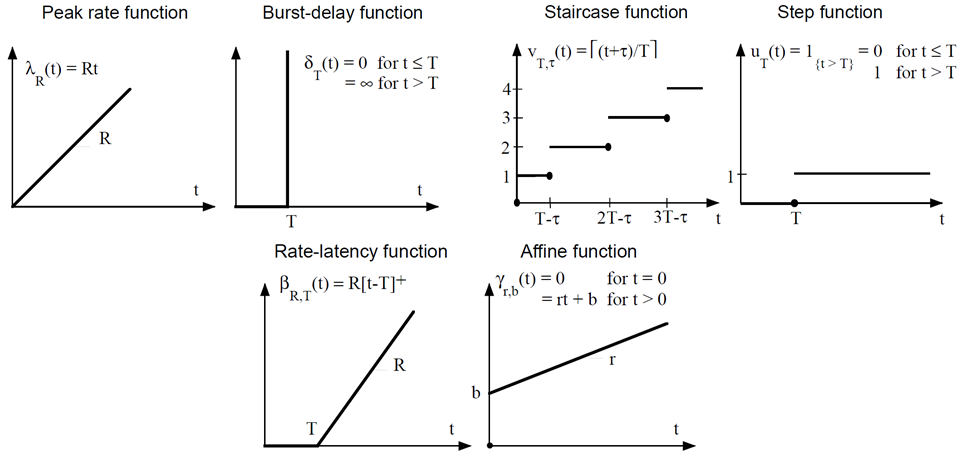
\includegraphics[width=0.95\textwidth]{figs/wsi.png}
	\caption{Example wide sense increasing functions, reprinted from \cite{NCBook}.}
	\label{fig:wsi}
\end{figure}

The main operations of min-plus calculus are the convolution and deconvolution operations, which act on sub-additive functions.  Convolution is a function of the form:
\begin{equation}
(f\otimes g)(t)\equiv inf_{\{0\leq s \leq t\}}\{f(t-s)+g(s)\}
\end{equation}
Note that if the functions $f,g$ are concave, this convolution simplifies into the computation of the minimum: 
\begin{equation}
(f\otimes g)(t)=min(f,g)
\end{equation}
Convolution in min-plus calculus has the properties of 
\begin{enumerate}
	\item closure: $(f\otimes g)(t) \in \mathpzc{F}$,
	\item Associativity,
	\item Commutativity, and
	\item Distributivity
\end{enumerate}

Similarly, deconvolution is a function of the form:
\begin{equation} 
(f\oslash g)(t)\equiv sup_{\{0\leq u\}}\{f(t+u)-g(u)\}
\end{equation}
Note that $\oslash$ is not closed in $\mathpzc{F}$ because $(f\oslash g)(t)$ is not necessarily $0$ for $t\leq0$.

% MORE INFO ABOUT NC
Network Calculus focuses on abstracting the network traffic and the
computing nodes as \textit{arrival curves} and traffic shaping
\textit{service curves}. The arrival curves and service curves model
the amount of data generated or serviced as functions of time window
size and are bounded by maximum and minimum arrival and service
curves.  By abstracting the network flows and traffic shapers as
arrival curves and service curves, respectively, (min,+) calculus can
be used to compose models of system behavior and calculate performance
characteristics of the application and the network.

Given an arrival function $R(t)$ for the data flow describing the
number of bits seen on the flow during the time interval $[0,t)$, the
arrival curve $\alpha$ constrains the flow if and only if
\begin{equation}
\forall s\leq t : R(t) -R(s) \leq \alpha(t-s)
\end{equation}
This relation is shown in Figure~\ref{fig:nc_arrival_curve}.
Intuitively the arrival curve representation transforms the data
production from a function of time, described by $R(t)$, into a
function of time-interval, described by $\alpha(t)$, for which $R\leq
R \otimes \alpha$.

\begin{figure}[htb]
	\centering
	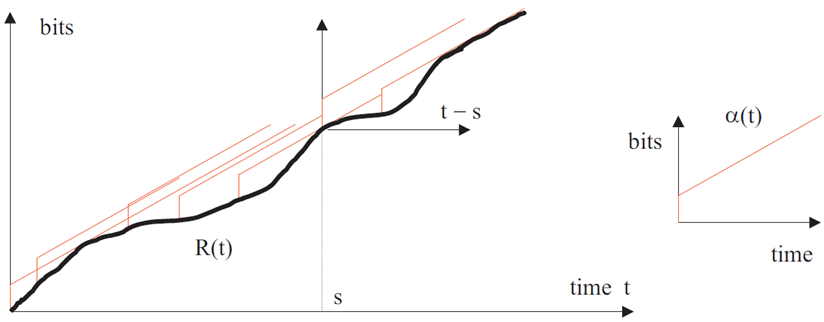
\includegraphics[width=0.95\textwidth]{figs/nc_arrival_curve.png}
	\caption{Illustrative example representing maximum arrival curves ($\alpha(t)$) for data flows ($R(t)$), reprinted from \cite{NCBook}.}
	\label{fig:nc_arrival_curve}
\end{figure}

Similarly, service curves transform the output data flow $R^*(t)$ into a minimum service curve $\beta$ according to the relation:
\begin{equation}
R(t)-R^*(t_0)\leq \beta(t-t_0), \forall t\geq 0\ \exists\  t_0\geq 0,t_0\leq t
\end{equation}
or more compactly $R^*\geq R\otimes\beta$.  This relation is shown in Figure~\ref{fig:nc_service_curve}.

\begin{figure}[htb]
	\centering
	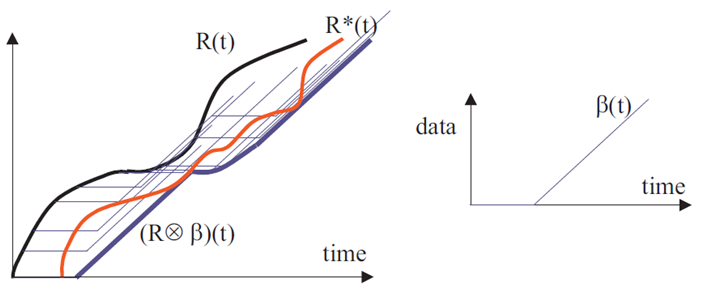
\includegraphics[width=0.95\textwidth]{figs/nc_service_curve.png}
	\caption{Illustrative example representing minimum service curves ($\beta(t)$) for output data flows ($R^*(t)$), reprinted from \cite{NCBook}.}
	\label{fig:nc_service_curve}
\end{figure}

From the input arrival curve $\alpha$ into a node providing service curve $\beta$, we can use Network Calculus to compute the output flow from the node and a few performance bounds governing the buffering delay and buffer requirements for the node.  The output flow from the node is constrained by the arrival curve $\alpha^* = \alpha\oslash\beta$.  Given the arrival curve and service curve for a node or system, we can compute the backlog and delay bounds, see Figure~\ref{fig:nc_bounds}; the backlog bound is given by:
\begin{equation}
R(t)-R^*(t)\leq sup_{\{s\geq 0\}}\{\alpha(s)-\beta(s)\}
\end{equation}
and the delay bound is given by: 
\begin{equation}
h(\alpha,\beta)=sup_{\{s\geq0\}}[inf\{T:T\geq0\ and\  \alpha(s)\leq\beta(s+T)\}]
\end{equation}

\begin{figure}[htb]
	\centering
	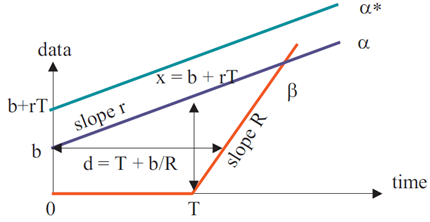
\includegraphics[width=0.75\textwidth]{figs/nc_bounds.png}
	\caption{Illustrative example representing the backlog and delay bounds calculated from input arrival curves and node service curves, reprinted from \cite{NCBook}.}
	\label{fig:nc_bounds}
\end{figure}

These bounds provide the requisite information needed to make design-time guarantees about \emph{worst-case} application performance on the network, given that both the application traffic profile and the system's network performance are deterministic. 

To enable compositional system analysis, Network Calculus allows for the concatenation of nodes, Figure~\ref{fig:nc_concatenation}, such that a flow traversing nodes $N_1$ and $N_2$ in sequence, where each node provides FIFO service curve $\beta_{i=1,2}$, the concatenation of the two nodes offers a service curve $\beta_1\otimes\beta_2$ to the flow.  A major advantage of this approach is the ability to "Pay Bursts Only Once" (PBOO), which is the property that the delay and buffer bounds are tighter when derived from the concatenation of the system than they would have been if they were calculated iteratively.  Again, note that this advantage is not applicable to non-FIFO systems\cite{NCBook}.  

\begin{figure}[htb]
	\centering
	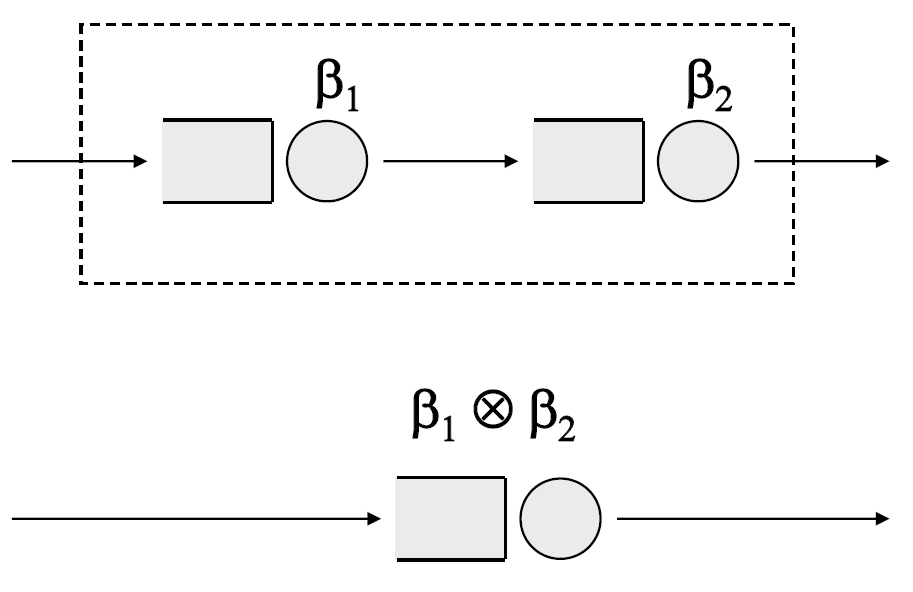
\includegraphics[width=0.75\textwidth]{figs/nc_concatenation.png}
	\caption{Illustrative example representing the concatenation of two nodes providing separate services into a single node providing an aggregate service.}
	\label{fig:nc_concatenation}
\end{figure}

However, the performance bounds calculated by Network Calculus are still worst-case performance based.  For instance, there is a temporal disconnect between the arrival/service curves and the actual performance of the application or the system.  This disconnect leads to analysis results that may still over-approximate the required buffer size or application delay on the network.  The cause of this over-approximation comes from the use of \emph{time windows}.  Because Network Calculus is focused on maximum data produced and minimum data serviced as functions of time window size, the time-varying nature of the data production or service is lost.  Despite an application producing a Bulk Data Transfer (BDT) during a period of high network resource availability, Network Calculus compares that BDT to all windows of time throughout the service time of the system.  As such, an expected drop in service during a different period of time will inadvertently negatively affect the application's predicted performance as analyzed by Network Calculus. 

\subsubsection{Real-Time Calculus}
Real-Time Calculus\cite{Thiele00real-timecalculus} builds from Network Calculus, Max-Plus Linear System Theory, and real-time scheduling to analyze systems which provide computational or communications services.  Unlike Network Calculus, Real-Time Calculus (RTC) is designed to analyze real-time scheduling and priority assignment in task service systems.  The use of (max,+)-calculus in RTC allows specification and analysis not of only the arrival and service curves described above for Network Calculus, but of upper and lower arrival curves ($\alpha^u(\Delta)$ and $\alpha^l(\Delta)$) and upper and lower service curves ($\beta^u(\Delta)$ and $\beta^l(\Delta)$).  These curves represent the miniumum and maximum computation requested and computation serviced, respectively.  An overview of RTC is given in Figure~\ref{fig:rtc_overview}.

\begin{figure}[htb]
	\centering
	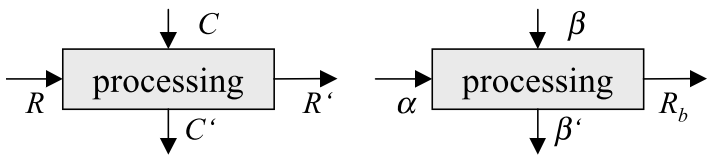
\includegraphics[width=0.75\textwidth]{figs/rtc_overview.png}
	\caption{Overview of Real-Time Calculus' request, computation, and capacity models.  $R(t)$ is the request function that represents the amount of computation that has been requested up to time $t$, with associated minimum request curve, $\alpha$.  $R'(t)$ is the total amount of computation delivered up to time $t$, with associated delivered computation bound $R_b(t)$.  $C$ and $C'$ are the capacity function and remaining capacity functions which describe the total processing capacity under full load and the remaining processing capacity, respectively.  $C$ and $C'$ are bounded by the delivery curve $\beta$ and the remaining delivery curve $\beta'$.}
	\label{fig:rtc_overview}
\end{figure}

RTC allows for the analysis of task scheduling systems by computing the request curve for a task model which is represented as a directed acyclic graph (DAG), the task graph $G(T)$.  The graph's vertices represent subtasks and each have their own associated required computation time $e(u)$, and relative deadline $d(u)$ specifying that the task must be completed $d(u)$ units of time after its triggering.  Two vertices in $G(T)$ may be connected by a directed edge $(u,v)$ which has an associated parameter $p(u,v)$ which specifies the minimum time that must elapse after the triggering of $u$ before $v$ can be triggered.  RTC develops from this specification the minimum computation request curve $\alpha_r$ and the maximum computation demand curve $\alpha_d$.  Finally, the schedulability of a task $T_i$ is determined by the relation:
\begin{equation}
\beta'(\Delta)\geq\alpha^i_d(\Delta)\ \ \ \forall\Delta
\end{equation}
which, if satisfied, guarantees that task $T_i$ will meet all of its deadlines for a static priority scheduler where tasks are ordered with decreasing priority.  Note that the remaining delivery curve $\beta'(\Delta)$ is the capacity offered to task $T_i$ after all tasks $T_{1\leq j<i}$ have been processed. Similarly to Network Calculus, RTC provides analytical techniques for the computation of performance metrics such as computation backlog bounds:
\begin{equation}
\text{backlog}\leq sup_{\{t\geq 0\}}\{\alpha^u(t)-\beta^l(t)\}
\end{equation}
which is equivalent to the network backlog bound derived in Network Calculus.  

\cite{RTCcomparison2011} compares different analytical methods for network performance analysis, namely Real-Time Calculus (RTC), probabilistic queuing models, parallel computation models, and protocol offload models.  The authors explain the current state of system evaluation, which is based predominantly on quantitative evaluation through simulation, but make the point that such simulation techniques should be used sparingly since \textit{only a finite state of initial states, environment behaviors, and execution traces can be considered by system simulators}.  The system which the authors model for their comparison is the case of Network Interface Cards (NICs) connected to a Local Area Network (LAN), for which they derive analytical bounds on the buffer requirements as they are affected by the input/output (I/O) subsystems, the network traffic, the NIC itself, and the memory controllers.  They point out that most researchers are still using Queuing Theory, in stochastic scenarios where the network traffic is modeled as random distributions of data.  Because RTC allows more precise descriptions of application traffic, it can be more beneficial for providing analysis of buffer requirements and delay experienced in the system.  RTC's ability to allow such specifications comes from its roots in Network Calculus and Max-Plus Linear System theory. 

\subsubsection{Stochastic Network Calculus}
% STOCHASTIC NETWORK CALCULUS
These deterministic constraints can be relaxed so that the deterministic arrival and service curves are instead replaced by stochastic processes, causing the bounds on the performance to be probabilistic as well\cite{Burchard06amin-plus}.  As described previously, these probabilistic performance bounds may not be precise enough to provide the types of guarantees required by certain classes of mission- or safety-critical systems.

\cite{SNC80211backlogdelay2011} provides a good description, system model, and analysis for stochastic Network Calculus applied to wireless networks.  In their work, they show the ability of network calculus to remove the need to make as many assumptions about the arrival or service processes (\emph{e.g.} exponential service distribution) to allow general arrival and service processes.  They apply stochastic network calculus to analyze backlog and delay bounds in 802.11 based multi-access systems.  They formally derive bounds for the backlog and delay in  the network and then compare these analytical results to bounds generated from network simulation using ns-2.  From this comparison, they conclude that the derived bounds are too loose and in fact get looser the closer the system gets to saturation.  They further conclude that this looseness is a direct result of stochastic network calculus itself, and claim that it requires further improvements.  It is important to remember what was stated previously by \cite{simulator_comparison_2003}: the simulation does not accurately model the dynamic behavior of real traffic, so the results from \cite{SNC80211backlogdelay2011} may too be inaccurate.  

Because Network Calculus deals with either deterministic worst-case application performance on a static network or stochastic application performance on a dynamic network, system designers and application designers under-utilize the network resources of systems which require strict design-time guarantees about application performance.  

\subsubsection{Extensions to Network Calculus}
% OTHER ADAPTATIONS AND ADDITIONS TO NC
When analyzing any complex system, the fidelity of the analysis results with respect to the actual system relies heavily on the level of detail of the models of the system's components and subsystems. \cite{Heidemann2001} covered the effects that different levels of detail have on analysis complexity and accuracy.  Importantly, they point out the requirement to not only be correct, but also be applicable, \emph{i.e.} analysis results should be both accurate with respect to the system being modeled, but should also be relevant for the analysis and development of real systems.  Additionally, they point out that not all systems require highly detailed modeling for the analysis results to be correct, since some systems and applications are insensitive to lower level details.

There are many efforts to make analytical techniques more representative of actual systems in order to increase the fidelity of the analysis results with respect to the run-time system.  The researchers in \cite{NCnetworkCoding} recognize the need to analyze not only the overall throughput of a network, but also the end-to-end delay experienced by information flows in the network.  Furthermore, they derive an analytical model of Wireless Network Coding\cite{networkcodingCOPE}, a technique for combining packets together for improving network throughput in wireless networks using broadcast techniques.  They show that by developing a model of the way the MAC layer works in the network and how the information flows are combined and disseminated, they can get tighter performance bounds and even derive methods for increasing performance in the network by altering the scheduling parameters of the packet flows.  Analyzing multiple performance parameters, in this case the network throughput and end-to-end delay, is a key element for analyzing and providing quality of service (QoS) to applications.

The authors in \cite{NCpacketcurve2012} also incorporate more precise models of the network to derive tighter performance bounds using Network Calculus.  They show that by modeling the packetization that occurs in the network using a \textit{packet operator} to transform arrival flows into packet flows, they can analytically derive tighter service curves than would be found from traditional Network Calculus.  Clearly, there exists a desire from application developers and system integrators to derive both accurate and precise design-time performance parameters for the system and its applications.  

Similarly, in \cite{NCspacewire}, the authors describe how to accurately model the SpaceWire network standard which has been developed for satellites in the European Space Agency (ESA).  Their network must be shared by both real-time (critical) and non real-time (non-critical) traffic, but the system developers require design-time guarantees about the temporal characteristics of all critical/real-time messages on the network.  Their work focuses on accurately representing the SpaceWire network, its (static) routing protocol, and the service profiles of its routers including the aspects of their flow control algorithms.  Building on previous work, they explain the need, for resource-constrained real-time systems, to accurately model the network traffic in order to derive a model of the network which is not too pessimistic.  They derive accurate Network Calculus/Real-Time Calculus (RTC) based models of the wormhole switches present in the network and show the fidelity of their analytical tools compared with the industrial simulation tools developed for SpaceWire networks.  Using a Network Calculus-based model, they are able to achieve analytical results that are the same order of magnitude as the simulation results for the critical traffic delay characteristics, but are less precise for the non-critical traffic in the network.  One important point they make that extends to all types of systems when comparing analysis and simulation techniques is this: \textit{worst-case delays can be extremely rare events which are hard to observe or recreate in simulations, but can be derived from analytical results.}\cite{NCspacewire}

Another approach to increasing the fidelity of the analysis is to model the Time Division Multiple Access (TDMA) medium channel access protocol using Network Calculus to derive performance metrics\cite{Schmitt2007}.  TDMA service curves are modeled such that the medium's transmit capacity is available to the node only during the node's designated slot.  During all other slots of the TDMA period, the medium's capacity is unavailable to the node and therefore the transmit capability of the node is zero.  As such, simple TDMA service curves can be described using simply a slot length, a slot bandwidth, and a TDMA period.

\cite{TDMA_Khan_98} analyzes the performance of TDMA with respect to the queue size for different probabilistic traffic models, and shows how the G/D/1 model with application-based probability distributions can be used to generate closed-form solutions for analyzing arbitrary traffic on a TDMA network.  

Another aspect of system design which has been gaining momentum is the development of self-adaptive systems which provide "self-*" properties such as self-management.  These types of systems are typically not used in CPS control applications or other systems which require real-time guarantees about timing or resource properties of the system.  The main reason for their absence from these types of systems and applications is the lack of available, accurate modeling and analysis techniques which properly capture the behavior of the applications in a way that allows the derivation of performance guarantees.  The authors in \cite{NCadaptivesystems} describe both the need for this type of analysis for these systems and describe the overview of how the analysis would work, based on concepts from Network Calculus.  Their main point is that currently such types of analysis tools do not exist for these systems, which makes developing the systems difficult with respect to these types of design parameters.  They propose developing a formalized standardization for the self-adaptive behavior, which they present as a state-space with available control actions based on the sensor data in the system. 

%%%%%%%%%%%%%%%%%%%%%%%%%%%%%%%%%%%%%%%%%%%%%%%%%%%%%%%%%%%%%%%%%%%%%%%%%%%%%%%%%%%
%%%%%%%%%%%%%%%%%%%%%%%%%%%%%%%%%%%%%%%%%%%%%%%%%%%%%%%%%%%%%%%%%%%%%%%%%%%%%%%%%%%
%%%%%%%%%%%%%%%%%%%%%%%%%%%%%%%%%%%%%%%%%%%%%%%%%%%%%%%%%%%%%%%%%%%%%%%%%%%%%%%%%%%
%%%%%%%%%%%%%%%%%%%%%%%%%%%%%%%%%%%%%%%%%%%%%%%%%%%%%%%%%%%%%%%%%%%%%%%%%%%%%%%%%%%
%%%%%%%%%%%%%%%%%%%%%%%%%%%%%%%%%%%%%%%%%%%%%%%%%%%%%%%%%%%%%%%%%%%%%%%%%%%%%%%%%%%
\section{Part 2: Run-Time Network Monitoring and Management}
\label{sec:related_part2}

In addition to design-time modeling and analysis, CPS system designers and integrators must ensure system stability during run-time by enforcing resource limitations on the applications to ensure no faulty or malicious code starves the system or other applications of network resources.  Such enforcement is the management of the network resource for the system.  Many different approaches exist to handle this type of management, generally falling into one of two categories: (1) static management or (2) dynamic management.  Static management of system resources is based around enforcement of resource allocations which were decided at design-time or deployment time.  Such management generally is associated with high-criticality systems which must be guaranteed.  Dynamic management of resources entails updating the resource allotments of each application based on currently available system resources and application load, and generally is in the class of adaptive management or adaptive systems (also called autonomic systems).  For this paper, we will address only static management of resources.  

Static management of network resources generally, but not necessarily, means applications are given a fixed set of resources for the lifetime of the system.  The part of the system which enforces these resource allotments however, may vary depending on the design of the system.  The enforcement may happen in the network layer, in the operating system kernel, or in some cases in the middleware facilitating the network communications for the applications.  We deem any enforcement happening in the kernel or in a lower layer to be \textit{infrastructural management} (since all applications on the system must use this infrastructure and are therefore managed by it).  We deem any resource management happening between the kernel and the application as \textit{middleware management}, since different applications deployed on the system may use different middleware stacks and therefore may be managed differently.  


\subsection{Infrastructural Approaches for Network Management}
\label{subsec:related_part2_infrastructural}

\cite{QT_Giambene2005}, Chapter 3 has a good overview of both IntServ and DiffServ.  DiffServ, for Differentiated Services, is designed for the provisioning of network resources to provide Quality of Service (QoS) to applications on the network but is unable to provide strict real-time guarantees about packet loss, delay, and bandwidth availability.  Instead, DiffServ was designed to scale well for large systems while still providing probabilistic guarantees.  IntServ, for Integrated Services, was designed to provide strict real-time guarantees about the QoS experienced by a flow on the network.  Unlike DiffServ, which does not maintain any state information in the routers along network flow paths, IntServ uses a resource reservation protocol (RSVP) with explicit setup of flows for deterministically allocating bandwidth and buffer space for a flow in each router along the flow's path.  While such an explicit out-of-band QoS reservation protocol enables similarly explicit resource availability and performance guarantees, the tradeoff comes in the ability of the system to scale to many nodes and many flows.  DiffServ's scalability comes from both the lack of explicitly maintaining per-flow state in the routers, by assigning traffic to a set of predefined classes, as well as using QoS assignment mechanisms which are built into the flow's messages, e.g. the DiffServ Code Point (DSCP) built into the Type of Service (ToS) byte in IPv4 headers and the Traffic Class byte of IPv6 headers.  

Both IntServ and DiffServ were originally designed for wired networks, but \cite{diffServ_intServ_Mahadevan1999} has worked on the required modifications to make them suitable for wireless networks, which have network connectivity and link characteristics which have more variance as a function of time.  The combination of low bandwidth, high loss, and node mobility require extensions to the QoS parameters and control options available to the application provided by the QoS infrastructures.  One such proposed extension is the loss profiles, which govern whether an application prefers dropping data in a bursty manner (as might be preferred by audio applications) versus a distributed manner (as might be preferred by video applications).  Similarly, since link bandwidth is typically much lower than in wired networks, IntServ/RSVP's refresh messages (used to determine network changes) should be sent with a lower frequency to provide as much network bandwidth as possible to application traffic.  In the same way, DiffServ requires modifications to support signaling information about link state and node location to overcome DiffServ's static provisioning scheme in the adaptation from wired to wireless networks.  

A system's network infrastructure may provide multiple different QoS provisioning implementations, such as both DiffServ and IntServ.  In this case, the applications can select which QoS provisioning to use.  Similarly, large networks may be grouped into subnets which each internally use different QoS provisioning schemes.  The boundaries between these subnets requires QoS mapping for flows which cross these boundaries.  Such mapping between QoS implementations and configurations is complex and makes providing guarantees about QoS for large complex networks challenging.  

Because both IntServ and DiffServ were designed for providing QoS to generic traffic for large networks including the internet, they were not designed to be able to provide performance guarantees to application developers.  As such, their design and implementation function more coherently in a system which has unknown applications and application load.  However, the classes of systems we focus on require more precise guarantees about performance and have the benefit of more precise design-time knowledge of applications and application load on the system.  

%TALK ABOUT QoS MODEL FOR MANET (3)
Flexible QoS Model for Mobile Ad-hoc Networks (MANETs), FQMM\cite{Xiao2000}, attempts to address the issue of run-time QoS management and adaptation to changing environmental conditions affecting the network.  Recognizing that both environmental and application behavior need to be taken into account for QoS management, they argue that two methods for providing QoS in the internet, IntServ\cite{Braden1994} and DiffServ\cite{Blake1998}, are not sufficient for dynamic mobile networks.  While IntServ's scalability problem will not affect dynamic mobile networks in the near future, they argue that the connection maintenance required by the Resource ReSerVation Protocol (RSVP) renders IntServ impractical.  DiffServ, on the other hand, might be able to provide long-term QoS to applications under the varying network conditions, but is not feasibly able to provide the kind of short-term QoS required by real-time applications.  Furthermore, DiffServ does not handle node mobility and external disturbances from the environment well as it was originally designed for relatively fixed (topologically) networks.  

To combat the issues in both IntServ and DiffServ, FQMM is designed to handle QoS for MANETs.  FQMM focuses on allowing for fine-grained provisioning of node resources and allowing node mobility through dynamically reassigning the roles of each of the nodes in the network.  The provisioning of the resources for flows in the network borrows ideas from both IntServ and DiffServ by combining the per-flow granularity of IntServ for high-priority flows while lower-priority flows are provisioned on a class basis as in DiffServ.  This differentiation between traffic classes and priority flows better utilizes the system resources to achieve the necessary performance for high priority flows which may need real-time performance.  To provide traffic shaping they constrain flows or classes to traffic profiles.  To combat the time-varying nature of the network, they instead define these traffic profiles as a percentage of the available network bandwidth.  This type of percentage-based flow constraint limits the adaptability of the network traffic however, as certain higher-priority real-time flows may have a minimum amount of bandwidth required that cannot be met with a percentile constraint on effective link bandwidth.  FQMM also addresses routing control to provide better run-time QoS to applications on the system.

\subsection{Middleware Based Approaches for Network Management}
\label{subsec:related_part2_middleware}

For system and application level adaptation to changing system resources, two main approaches, namely fixed reservation of flows and run-time adaptation, provide benefits for performance or resilience.  These two approaches cannot be used alone however, as fixed reservation of flows based on design-time network analysis causes low resource utilization and run-time adaptation is generally not prepared for excessive congestion or other disturbances.  GARA \cite{Foster2000} combines these two paradigms to provide more graceful degradation and higher resource utilization at the system and application level.  GARA uses priority based flow reservation which can be altered at run-time by both the application and by third parties on behalf of the application.  This type of reservation scheme allows applications to monitor and react to changes in network capacity, while still attempting to ensure that high-priority flows can traverse the network.  Furthermore, this type of reservation scheme is more amenable to dynamic flows which may only be active during a portion of time that the system is active.  Statically defined slots reserved at design-time cause wasted resources by these applications whose flow is reserved but not used the entire time.  

%DDS QoS options; need other examples

Finally, there do exist different protocols and communications paradigms which support run-time control of application network traffic, such as the Quality of Service (QoS) control mechanisms present in many implementations of OMG's Data Distribution Service (DDS) standard\cite{OMG-DDS:07}\cite{OpenDDS:07}.  However, often the mechanisms available for controlling the QoS parameters of a given data stream are complex, interacting mechanisms which may be difficult for the application developer to understand and therefore are also not amenable to modeling and analysis at design time\cite{Hoffert:2010:AED:1862821.1862825}.  Furthermore, the developers may not be provided with or have control over lower level implementation details such as the selected transport layer protocol, which may affect the available QoS or may not be fully supported by the infrastructure.  Additionally, many of the available interaction paradigms either do not support design time QoS analysis with run-time monitoring and control or the supported QoS analysis and control interfaces are only informally specified.
